\chapter{Ανάλογα ποσά - Αντιστρόφως ανάλογα ποσά}
\begin{exercise}
Να σχεδιάσεις ένα ορθοκανονικό σύστημα ημιαξόνων, με μονάδα το 1 cm και να
τοποθετήσεις τα σημεία Α(2,3), Β(3,2), Γ(4,5), Δ(5,5), Ε(1,4), Z(7,3), Η(7,2), Θ(6,2),
Ι(6,0), Κ(0,5). Τι παρατηρείς για τα σημεία Ι και Κ; Πού βρίσκονται αυτά; Μπορείς να
γενικεύσεις τις παρατηρήσεις σου για τα σημεία που έχουν τετμημένη ή τεταγμένη το
μηδέν;
\end{exercise}
\begin{lstlisting}
import matplotlib.pyplot as plt

plt.clf()
points = [(2,3), (3,2), (4,5), (5,5), (1,4), (7,3), (7,2), (6,2), (6,0), (0,5)]
pointName = ['Α','Β','Γ','Δ','Δ','Ε','Ζ','Η','Θ','Ι','Κ']
x = [p[0] for p in points]
y = [p[1] for p in points]
color=['m','g','r','b']
plt.grid()
plt.scatter(x,y, s=100 ,marker='o', c=color)
for (i,p) in enumerate(points):
    plt.annotate(pointName[i],(p[0],p[1]))

plt.show()
\end{lstlisting}
\begin{figure}
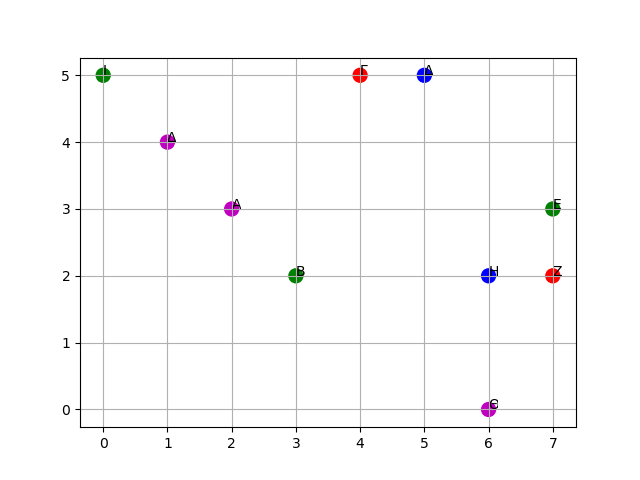
\includegraphics{graph1.png}
\end{figure}
\begin{exercise}
\sel[2]{89}
Σε ορθοκανονικό σύστημα ημιαξόνων να τοποθετήσεις τα σημεία Α(2,1), Β(1,2), Γ(2,3)
και Δ(3,2). Τι σχήμα είναι το ΑΒΓΔ; Αν τα ευθύγραμμα τμήματα ΑΓ και ΒΔ τέμνονται
στο σημείο Κ, ποιες είναι οι συντεταγμένες του Κ;
\end{exercise}
\begin{lstlisting}
import matplotlib.pyplot as plt

plt.clf()
points = [(2,1), (1,2), (2,3), (3,2)]
pointName = ['Α','Β','Γ','Δ']
x = [p[0] for p in points]
y = [p[1] for p in points]
color=['m','g','r','b']
plt.grid()
plt.scatter(x,y, s=100 ,marker='o', c=color)
for (i,p) in enumerate(points):
    plt.annotate(pointName[i],(p[0],p[1]))

x = [points[0][0],points[2][0]]
y = [points[0][1],points[2][1]]
plt.plot(x,y)
x = [points[1][0],points[3][0]]
y = [points[3][1],points[3][1]]
plt.plot(x,y)

plt.show()
\end{lstlisting}
\begin{figure}
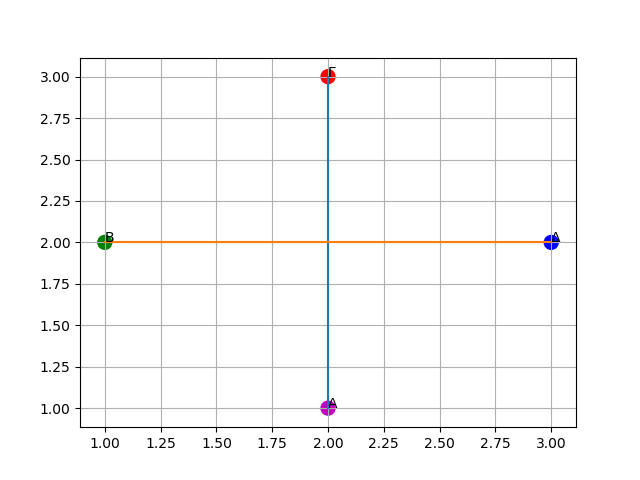
\includegraphics{graph2.png}
\end{figure}

\begin{exercise}
\sel[3]{89}
Γράψε πέντε διατεταγμένα ζεύγη σημείων, των οποίων η τετμημένη τους είναι ίση με
την τεταγμένη τους. Μπορείς να τα
τοποθετήσεις, σε ένα ορθοκανονικό
σύστημα ημιαξόνων; Τι παρατηρείς;
\end{exercise}
\begin{lstlisting}
import matplotlib.pyplot as plt

plt.clf()
points = [(1,1), (2,2), (5,5), (10,10), (15,15)]
pointName = ['Α','Β','Γ','Δ','Ε']
x = [p[0] for p in points]
y = [p[1] for p in points]
color=['m','g','r','b']
plt.grid()
plt.scatter(x,y, s=100 ,marker='o', c=color)
for (i,p) in enumerate(points):
    plt.annotate(pointName[i],(p[0],p[1]))

plt.show()
\end{lstlisting}
\begin{figure}
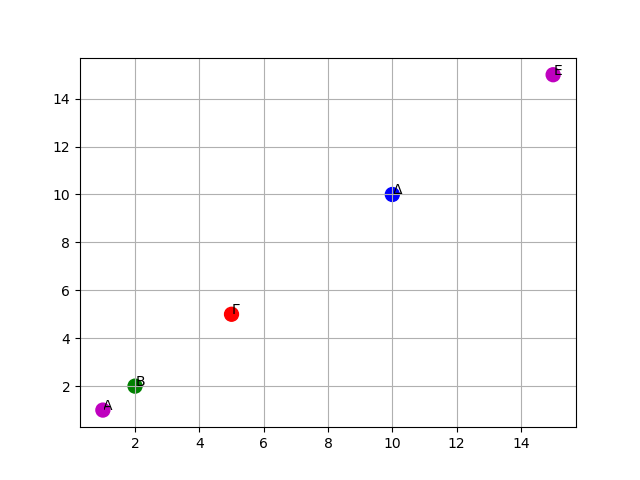
\includegraphics{graph3.png}
\end{figure}

\begin{exercise}
\sel{90}
Συμπλήρωσε τον παρακάτω πίνακα:
\begin{table}
\begin{tabular}{|l|c|c|c|}
Πλευρά τετραγώνου& 1,5 cm& 4 cm& 4,5 cm\\\hline
Περίμετρος τετραγώνου&&&\\\hline
\end{tabular}
\end{table}
\begin{itemize}
\item Εξήγησε πώς προκύπτουν οι αριθμοί της δεύτερης σειράς.
\item Βρες για κάθε τετράγωνο το κλάσμα πλευρά προς περίμετρο.
\item Ποιο είναι το συμπέρασμα που βγάζεις;
\end{itemize}
\end{exercise}
\begin{lstlisting}
>>> 4*1.5
6.0
>>> 4*4
16
>>> 4*4.5
18.0
\end{lstlisting}
\begin{tabular}{|l|c|c|c|}
Πλευρά τετραγώνου& 1,5 cm& 4 cm& 4,5 cm\\\hline
Περίμετρος τετραγώνου&6&16&18\\\hline
\end{tabular}
Θυμηθείτε το ποσοστό σε κλάσμα:
\begin{lstlisting}
def posostoseklasma(fx):
    fx = float(fx)
    denom = 100
    while int(fx) != fx:
         fx *= 10
         denom *= 10
    fx = int(fx)
    return(Fraction(fx,denom))
\end{lstlisting}
Το fx είναι είναι ο αριθμητής ενός κλάσματος με παρονομαστή 100. Εδώ δεν θα υπάρχει ο παρονομαστής 100 οπότε έχουμε denom = 1.
\begin{lstlisting}
def posostoseklasma(fx):
    fx = float(fx)
    denom = 1
    while int(fx) != fx:
         fx *= 10
         denom *= 10
    fx = int(fx)
    return(Fraction(fx,denom))

posostoseklasma(1.5/6)
posostoseklasma(4/16)
posostoseklasma(4.5/18)
\end{lstlisting}
και το αποτέλεσμα είναι:
\begin{lstlisting}
>>> posostoseklasma(1.5/6)
Fraction(1, 4)
>>> posostoseklasma(4/16)
Fraction(1, 4)
>>> posostoseklasma(4.5/18)
Fraction(1, 4)
\end{lstlisting}
Άρα παντού το κλάσμα είναι $\frac{1}{4}$.
\begin{exercise}
\sel{90}
Χρησιμοποιούμε τη φωτογραφική μηχανή
για να απεικονίσουμε εικόνες αντικει-
μένων. Οι εικόνες αυτές δείχνουν τα
πραγματικά αντικείμενα σε σμίκρυνση.
Στη φωτογραφία το ύψος ενός παιδιού
είναι 2 cm ενώ γνωρίζουμε ότι το πραγμα-
τικό του ύψος είναι 1,65 m = 165 cm. Πόση θα είναι τότε η σμίκρυνσή του
στη φωτογραφία;
\end{exercise}
\begin{lstlisting}
>>> 2/165
0.012121212121212121
\end{lstlisting}

\begin{exercise}
\sel{91}
Μετρούμε μια απόσταση, σε χάρτη, με κλίμακα 1:10.000.000 και τη βρίσκουμε
ίση με 2,4 cm. Ποια είναι η πραγματική απόσταση των δύο σημείων;
\end{exercise}
\begin{lstlisting}
>>> x = 2.4*10000000
>>> x
24000000
>>> x = x/100
>>> x
240000
>>> x = x/1000
>>> x
240
\end{lstlisting}
240Km